\documentclass[a4paper,12pt]{article}
\usepackage{graphicx}
\usepackage{enumerate}
\usepackage{geometry}
\usepackage{times}
\geometry{legalpaper, portrait, margin=.75in}

\begin{document}

\begin{flushright}

\vspace{1.1cm}

{\bf\Huge Lab 2}

\rule{0.25\linewidth}{0.5pt}

\vspace{0.5cm}
%Put Authors
Justin Ely
\linebreak
\newline
%Put Author's affiliations
\footnotesize{615.202.81.FA15 Data Structures \\}
\vspace{0.5cm}
% Date here below
27 October, 2015
\end{flushright}

\noindent\rule{\linewidth}{1.0pt}

%%%%%%%%%%%%%%%%%%%%%%%%%%%%%%%%%%%%%%%%%%%%%%%%%%%%%%%%%%

\section{Comments}
In many senses, a matrix is just a specialized array with different (and additional) mathematical operations.  Thinking this way, 
it's a seamless transition to implement a matrix type with an underlying array.  Random access to the array gives the power to quickly, 
$O(1)$, access elements as is necessary in many of the matrix functions.  Additionally, the inherent multi-dimensional shape of the 
matrix can be mirrored in the array, something not available in other data structures.  In other 1D structures, the 2D indices would need
to be stored as metadata to the actual data values themselves instead of being inherent in the array indices. 

However, beyond the natural extension of array to matrix, the core array data structure lends little benefit to some of the most costly
methods implemented.  The Minor method, used as part of the Determinate, requires iterating over every element of the input array
and thus gains no benefit from the random-access of the array.  Such an implementation would see similar performance from a
linked implemenation, where iterating is a necessity.  

\subsection{Iterative}
An iterative solution isn't very well suited to this problem as the solution is well-expressed (and given) recursively.  This means
an iterative solution needs to be worked out and tested from the initial recursive definition, which takes additional time and effort. 

However, in this case an iterative solution could be done without too much trouble: iterating from the initial order down to 1, removing
rows/columns and continuing to add terms to the determinate calculation.  In this case, I would strongly consider a linked-list implementation.  
A linked structure would allow deletion of all elements in a row/column on each iteration, whereas this would be much more difficult in an array of fixed size.  
This would decrease the space complexity, as the space required would actually decrease with each successive call, but increase the
time complexity as some terms in the determinate calculation benefit from random access and would now require iteration. 


%%%%%%%%%%%%%%%%%%%%%%%%%%%%%%%%%%%%%%%%%%%%%%%%%%%%%%%%%%

\section{Design}
Much of the design was limited by the supplied requirements: an array data structure using a recursive call for calculating the determinate.  However, limitations and enhancements to the specific design employed are discussed below.


\subsection{Limitations}
The Matrix class is limited to only integer types of the standard int precision.  A matrix, in abstract, is not limited to integers and works just as 
well with floating-point numbers.
For the current purposes, the required input was limited to integers, so only an integer constructor and methods were added. 

The Determinate method, however, is limited by long-integer precision.  For orders beyond 6, development quickly showed that
the standard int precision wasn't sufficient.  Therefore a long-int precision was implemented instead.  However, this still limits the final
determinate calculation, though to a higher value than int.  

As discussed in the Efficiency section, the current algorithms employed are a major limiting factor in the actual usefulness of the 
current implementation.  The determinate for matrices of order 13 take $\sim$30 minutes to calculate, which severely limits the usefulness
of the code. 

\subsection{Enhancements}
Though not entirely an enhancement, the given requirements only specify a maximum matrix order of 6, and the design employed
allows an arbitrary matrix size.  This arbitrary size is only realistically useful up to order $\sim$10, after which the evaluation time
becomes prohibitive. 

Arguably an enhancement, the main driver's file parsing is able to handle very poorly formatted input matrices.  The only requirement 
is for a first integer $(n)$ followed by $n^2$ integers.  The first integer is evaluated as the matrix order, and the following values are 
inserted in row-major order.  This means they could be input all as a single line, each on newlines, or anything in-between so long as
the number of values is equal to $o^2$.  This is only {\it arguably} an enhancement as, in certain circumstances, this could be seen as
a limitation in not checking for properly formatted row/column data.  For the current requirements, this was deemed not a concern, and in
many implementations such a flexible input format could be a benefit.

An additional enhancement was the implementation of a Print() method for the matrix.  Very useful for debugging and 
verification, the simple method was perhaps the most useful addition during the development. phase


%%%%%%%%%%%%%%%%%%%%%%%%%%%%%%%%%%%%%%%%%%%%%%%%%%%%%%%%%%

\section{Efficiency}
The efficiency of the determinate calculation is limited most by the method employed to find the minor matrix, as the 
random access of the array implementation allows O(1) operations for other two terms of the Determinate calculation.
The Minor method needs to iterate over every element of the input matrix, copying it's value into the output matrix (while 
skipping the row, column for which the matrix is to be determinate).  Thus, a single minor call is of $O(n^2)$, but a 
recursive call to Determinate will need to calculation the minor N times. 

To test the real-world complexity of the determinate calculation, timing functionality was added to test the actual time required
to calculate the determinate of each order. The results, as well as a fit to the data, can be seen in Figure 1.  From this analysis, we
can see that the time-complexity is exponential, $O(10^n)$, and grows significantly which each successive order. 
 For the system used for testing (2.8Ghz Intel Core i7), the determinate of the matrix order 13 took $\sim$30 minutes to evaluate.

\begin{figure}[h]
    \centering
    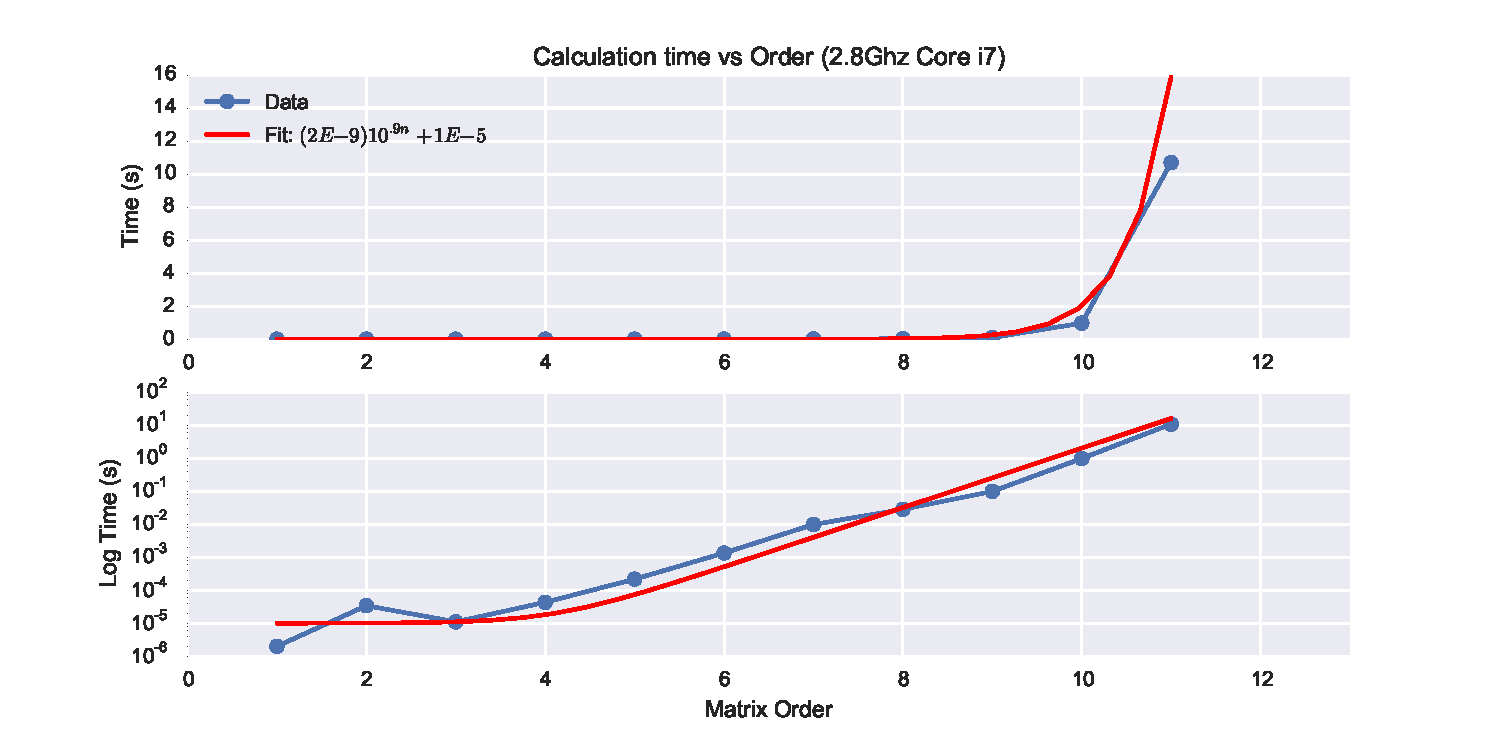
\includegraphics[width=.9\textwidth]{time_complexity.pdf}
    \caption{Time complexity of the determinate method.  Top subplot shows the data and fit on a linear y-scale, where the bottom plot shows
    the same data on a logarithmic y-scale.  Note the variation in behavior at low-order.}
    \label{fig:mesh1}
\end{figure}

Real-world evaluation of space complexity was difficult to evaluate directly, so a theoretical calculation was done instead.  Each call to the
minor method created a new array of $(n-1) * (n-1)$ elements, which leads to a growth in required size with each step.
This could potentially be made more efficient by implementing a strategy that doesn't require creating a new copy of the array for
each recursive call.  Something that masked-out the deleted rows/columns could perform the same calculation with a constant space
requirement.

\begin{figure}[h]
    \centering
    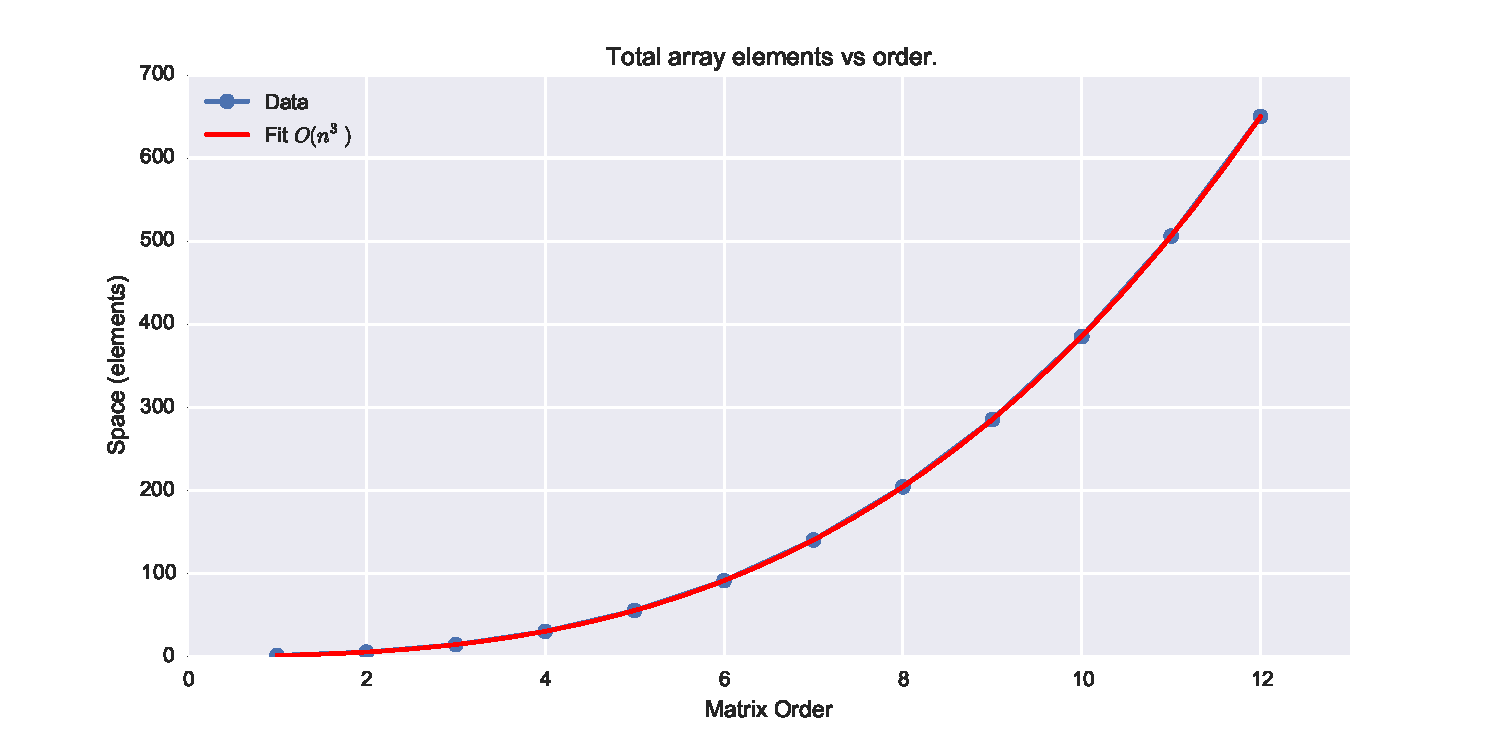
\includegraphics[width=.9\textwidth]{space_complexity.pdf}
    \caption{Space complexity of the determinate method.  The behavior shown is calculated, not observed, and is well fit by
     an $O(n^3)$ polynomial.}
    \label{fig:mesh1}
\end{figure}


%%%%%%%%%%%%%%%%%%%%%%%%%%%%%%%%%%%%%%%%%%%%%%%%%%%%%%%%%%

\section{What I learned}
In this lab, the most impactful thing I learned was the true, real-world, cost of exponential growth algorithms.  A small matrix
determinate can be evaluated in nanoseconds, but increase just a single order of magnitude and nanoseconds quickly becomes
minutes, hours, and days.  Thus, the algorithm employed here quickly becomes useless in any real-world setting beyond a moderate
sized matrix.  Spending time on finding the most efficient algorithm can save orders of magnitude more time down the road.  A corollary
of this is that small-number tests can hide the inefficiency of algorithms, and special attention must be paid to fully exercise an implementation.  
If my tests never went beyond order 6, this cost would not have been fully understood.

%%%%%%%%%%%%%%%%%%%%%%%%%%%%%%%%%%%%%%%%%%%%%%%%%%%%%%%%%%

\section{Next time}
In a future implementation, I'd like to add more methods to the matrix object to support common operations.  Operations such
as transpose, add, subtract, multiply, and divide are commonly used methods that would make the matrix much more useful
to an end-user.  Additionally, allowing floating-point numbers in the matrix would be a considerable advantage to real-word use.

Perhaps the most useful change I'd like to make would be to the Minor method itself.  The algorithm implemented here is 
very brute-force, with no attempt at optimization, and is very slow for even moderately sized matrices.  Next time, I'd devote 
more effort into researching and implementing alternate Minor algorithms that have better time efficiency (should one exist).


%%%%%%%%%%%%%%%%%%%%%%%%%%%%%%%%%%%%%%%%%%%%%%%%%%%%%%%%%%

\end{document}
